\section{Integrali doppi e tripli (analisi II)}
\rule{\textwidth}{2pt}
\subsection{Integrali doppi}
L'integrale doppio serve per il calcolo di volumi.\newline
\[
    \int_{\Omega} f(x,y) dxdy
\]
Proprietà:
\begin{itemize}
    \item se $f(x,y)\geq g(x,y) \Rightarrow \int_\Omega f(x,y) dxdy \geq \int_{\Omega} g(x,y)dxdy$
    \item $|\int_{\Omega}f(x,y) dxdy| \leq \int_{\Omega}|f(x,y)|dxdy$
    \item linearità:
    \[
        \int_{\Omega}[\alpha \cdot f(x,y) + \beta \cdot g(x,y)]dxdy = \alpha \int_{\Omega} f(x,y) dxdy + \beta \int_{\Omega} g(x,y) dxdy
    \]
    \item addittività: Se $\Omega_1, \Omega_2$ sono aperti tali che $\Omega_1 \cap \Omega_2 = \O$, allora
    \[
        \int_{\Omega_1 \cap \Omega_2}f(x,y)dxdy = \int_{\Omega_1} f(x,y) dxdy + \int_{\Omega_2} f(x,y) dxdy
    \]
    \item valor medio: se $f \in C^0(\Omega)$ con $\Omega$ chiuso e limitato, allora esiste $(x_0, y_0) \in\Omega$ tale che 
    \[
        f(x_0, y_0) = \frac{1}{|\Omega|}\int_{\Omega}f(x,y)dxdy
    \]
\end{itemize}
\ \newline
\textbf{Regione y-semplice:} Se l'intersezione di una qualunque retta verticale con la $\Omega$ è un segmento o vuota.\newline
\textbf{Regione x-semplice:} Se l'intersezione di una qualunque retta orizzontale con la $\Omega$ è un segmento o vuota.\newline
\newline
Una regione piana $\Omega$ si dice \textbf{regolare} se può essere scomposta in un numero finito di regioni semplici.
\subsubsection{Integrale su una regione semplice}
Consideriamo il caso in cui $\Omega$ è un rettangolo con vertici $a, b, c, d$.\newline
Prendendo una sezione verticale rispetto a $x$ nel punto $x_0$, notiamo che l'area è rappresentata da $A = \int_{c}^{d}f(x_0, y)dy$. Variando per tutte le $x_0$ che appartengono all'intervallo $[a,b]$ otteniamo
\[
    \int_{a}^{b} \left(\int_{c}^{d}f(x,y) dy \right)dx
\]
Questo concetto è applicabile anche a tutte le $\Omega$ semplici, l'area della sezione rispetto a $x$ è $A = \int_{g(x)}^{h(x)}f(x,y)dy$, e quindi il volume:
\[
    \int_{a}^{b}\left(\int_{g(x)}^{h(x)}f(x,y) dy \right)dx
\]
Dunque:\newline
\textbf{teor.} Formula di riduzione per integrali doppi:
\begin{itemize}
    \item Se $\Omega$ è \textbf{y-semplice}, cioè se $\Omega = \{(x,y) \in \mathbb{R}^2, a< x<b, g(x)<y<h(x)\}$
    \[
        \int_{\Omega}f(x,y)dxdy = \int_{a}^{b}\left(\int_{g(x)}^{h(x)}f(x,y)dy\right)dx
    \]
    Dove $g(x)$ rappresenta il limite inferiore di $\Omega$, e $h(x)$ il limite superiore.
    \item Se $\Omega$ è \textbf{x-semplice}, cioè se $\Omega = \{(x,y) \in \mathbb{R}^2, a< y<b, g(x)<x<h(x)\}$
    \[
        \int_{\Omega}f(x,y)dxdy = \int_{a}^{b}\left(\int_{g(y)}^{h(y)}f(x,y)dx\right)dy
    \]
    Dove $g(x)$ rappresenta il limite inferiore di $\Omega$, e $h(x)$ il limite superiore.
\end{itemize}
Questo teorema afferma che, su una regione semplice, un integrale doppio si può calcolare con due integrazioni successive. Se poi la regione fosse regolare ma non semplice, si può scomporre in un numero finito di regioni semplici sulle quali applicare questo teorema e concludere sommando tutti i risultati.
\subsubsection{Cambio di variabili}
Il problema è quello di trasformare un insieme $\Omega \subset \mathbb{R}^2$ in un altro insieme $T \subset \mathbb{R}^2$ più semplice geometricamente.
\[
    (u,v) = \Phi(x,y)   
\] 
La trasformazione $\Phi$ deve essere biunivoca, cioè all'interno dell'intervallo la derivata prima di $\Phi$ non deve annullarsi.\newline
Stiamo quindi cercando di creare una trasformazione $\Phi: \Omega \rightarrow T$ che sia invertibile
\[
    \Phi : \begin{cases}
        u = u(x,y)\\
        v = v(x,y)
    \end{cases}
\]
\[
    \Phi^{-1} : \begin{cases}
        x = x(u,v)\\
        y = y(u,v)
    \end{cases}
\]
Cerchiamo ora una condizione sulle derivate di $\Phi$ in modo da essere sicuri che il cambio di variabile sia invertibile.\newline
\newline
Sia $\Phi : \Omega \rightarrow  T$ una trasformazione piana con componenti $u = (x,y)$ e $v = v(x,y)$ di classe $C^1$. Si chiama \textbf{matrice Jacobiana} della trasformazione $\Phi$ la matriche
\[
    \frac{\delta(u,v)}{\delta(x,y)} = \left[\begin{matrix}
        u_x(x,y) & u_y(x,y)\\
        v_x(x,y) & v_y(x,y)
    \end{matrix}\right]
\]
Se risulta $det\left(\frac{\delta(u,v)}{\delta(x,y)}\right) \neq 0 \;\; \;\forall\;(x,y) \in \Omega$(senza la frontiera), allora $\Phi$ sarà localmente invertibile. A differenza del caso monodimensionale, questa condizione non consente però di concludere che $\Phi$ sia globalmente invertibile. Inoltre se questa condizione è valida, sappiamo che di sicuro anche per la matrice Jacobiana della funzione inversa $\Phi^{-1}$ vale $det\left(\frac{\delta(x,y)}{\delta(u,v)}\right) \neq 0 \;\; \;\forall\;(u,v) \in T$. Inoltre questa condizione di non annullamento viene garantita solo nell'insieme aperto.\newline
\newline
Il termine $det\left(\frac{\delta(x,y)}{\delta(u,v)}\right)$ rappresenta il fattore che dilata o contrae l'elemento d'area, dunque abbiamo:
\[
    dxdy = det\left(\frac{\delta(x,y)}{\delta(u,v)}\right)dudv
\]
\textbf{teorema del cambiamento di variabili negli integrali doppi}\newline
Sia $\Omega \in \mathbb{R}^2$ un aperto limitato regolare e sia $\Phi : \Omega \rightarrow T$ una trasformazione piana invertibile di classe $C^1$. Allora, detta $\Phi^{-1}$ la sua inversa, se vale $det\left(\frac{\delta(u,v)}{\delta(x,y)}\right) \neq 0 \;\; \;\forall\;(x,y) \in \Omega$, allora vale anche $det\left(\frac{\delta(x,y)}{\delta(u,v)}\right) \neq 0 \;\; \;\forall\;(u,v) \in T$. Sia poi $f \in R(\Omega)$; allora
\[
    \int_\Omega f(x,y) dx dy = \int_T f(x(u,v), y(u,v)) \cdot \left|det\left(\frac{\delta(x,y)}{\delta(u,v)}\right)\right| du dv
\]
\subsubsection{Cambio di variabili in coordinate polari}
Sia $\Omega \in \mathbb{R}^2$, i punti $(x,y)$ vengono trasformati in punti $(\rho, \theta) \in T$ tali che
\[
    \Phi^{-1} : \begin{cases}
        x = \rho cos(\theta)\\
        y =\rho sin(\theta)
    \end{cases}
\]
\[
    \rho = \sqrt{x^2 +y^2} \geq 0 \quad \quad \theta \in[0, 2\pi)
\]
Questa trasformazione trasforma il piano $\mathbb{R}^2$ in una striscia di piano, la cui altezza massima è $\theta = 2\pi$ (non compresa) e la lunghezza è determinata da $\rho$.\newline
\newline
Un caso particolare è rappresentato da $\rho = 0$, in cui $\theta$ non è definito.\newline
\newline
Analiziamo il Jacobiano:
\[
    \text{Jacobiano}\;= \rho
\]
Nelle integrazioni in coordinate polari, essendo il Jacobiano = $\rho$, il termine $dx \; dy$ diventa $\rho \; d \rho \; d \theta$.\newline
\newline
Il cambio in coordinate polari è consigliabile quando nell'integranda compare l'espressione $x^2 + y^2$.
\subsection{Integrali tripli}
Ridurre un integrale triplo significa scomporre $3 = 1+2$ o $3=2+1$,cioè svolgere prima un integrale semplice e poi un integrale doppio o viceversa.\newline
Salvo pochi casi in cui si può operare in entrambi i modi, la scelta dipenderà dalla forma dell'insieme di integrazione.
\subsubsection{Integrazione per fili}
Se l'insieme $\Omega$ è semplice rispetto all'asse $z$ o \textbf{z-semplice}, cioè esistono $D \subset \mathbb{R}^2$ e $g,h \in C^0(\bar{D})$ tali che $g<h$ in $D$ e
\[
    \Omega = \{(x,y,z) \in \mathbb{R}^3, (x,y)\in D, g(x,y)<z<h(x,y)\}
\]
cioè se l'intersezione di una retta parallela all'asse $z$ e $\Omega$ è un segmeno o vuota, allora data $f \in C^0(\Omega)$ si ha
\[
    \int_\Omega f(x,y,z) dxdydz = \int_D\left(\int_{g(x,y)}^{h(x,y)}f(x,y,z) dz\right)dxdy
\] 
Allo stesso modo si procede nel caso di $\Omega$ x-semplice o y-semplice.\newline
\newline
Ma non tutti i domini sono semplici rispetto a una delle tre variabili, per cui\dots
\subsubsection{Integrazione per strati}
Se $\Omega$ è semplice rispetto alla coppia $(x,y)$ e cioè esistono $a<b$ tali che
\[
    \Omega = \{(x,y,z) \in \mathbb{R}^3, a<z<b, (x,y) \in D_z \;\forall\;z \in(a,b)\}
\]
dove $D_z$ è un insieme regolare $\;\forall\;z \in(a,b)$, cioè se l'intersezione fra un piano parallelo al piano $z=0$ e $\Omega$ è un insieme regolare oppure è vuota, allora data $f \in C^0(\bar{\Omega})$ si ha 
\[
    \int_\Omega f(x,y,z) dxdydz = \int_{a}^{b}\left(\int_{D_z}f(x,y,z)dxdy\right)dz
\]
Allo stesso modo si procede nel caso di $\Omega$ semplice rispetto alle coppie $(x,z)$ o $(y,z)$.
\subsubsection{Cambio di variabili}
ANche le formule di cambio di variabili negli integrali tripli si ricavano senza sorprese rispetto a quelle per gli integrali doppi.
\subsubsection{Cambio di variabili in coordinate cilindriche}
Le coordinate cilindriche sono le coordinate polari con una dimensione invariante (la $z$) in più.\newline
\newline
Presa una sezione verticale (cioè di un piano che passa per l'asse $z$) si definiscono:
\begin{itemize}
    \item $\rho$ rappresenta la distanza tra l'origine degli assi e la proiezione del punto P sul piano $xy$ (in poche parole la distanza fra il punto e l'asse $z$).
    \item $z$ rappresenta la quota del punto $P$ dal piano $xy$.
    \item $\theta$ di quando deve ruotare il piano per rappresentare il volume di partenza.
\end{itemize}
\[
    \;\forall\; \begin{cases}
        \rho \in [0,\infty)\\
        \theta \in [0,2\pi)\\
        z \in \mathbb{R}
    \end{cases} \;\; \Longrightarrow \begin{cases}
        x = \rho cos(\theta)\\
        y = \rho sin(\theta)\\
        z = z
    \end{cases}
\]
Matrice Jacobiana:
\[
    \frac{\delta(x,y,z)}{\delta(\rho,\theta,z)} = \left[
    \begin{matrix}
        cos(\theta) & -\rho sin(\theta) & 0\\ 
        sin(\theta) & \rho cos(\theta) & 0 \\ 
        0 & 0 & 1
    \end{matrix}\right]
\]
\[
    det\left(\frac{\delta(x,y,z)}{\delta(\rho,\theta,z)}\right) = \rho 
\]
Il fattore di variazione del volume è quindi $\rho$ e si annulla solo sull'asse $z$ che è parte della prontiera dell'insieme dove variano $(\rho,\theta,z)$.
\subsubsection{Cambio di variabili in coordinate sferiche}
\begin{center}
    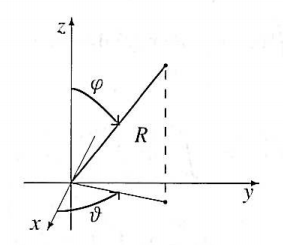
\includegraphics[height=5cm]{../6-integrali doppi e tripli (analisi II)/img1.PNG}
\end{center}
\[
    \;\forall\; \begin{cases}
        \rho \in [0,\infty)\\
        \phi \in [0,\pi]\\
        \theta \in [0,2\pi)
    \end{cases} \;\; \Longrightarrow \begin{cases}
        x = \rho sin(\phi) cos(\theta)\\
        y = \rho sin(\phi) sin(\theta)\\
        z = \rho cos(\phi)
    \end{cases}
\]
\[
    \rho^2 = x^2 +y^2+z^2 \;\; \text{e rappresenta la distanza fra il punto $(x,y,z)$ e l'origine}\;
\]
\ \newline
oppure, se si prende $\phi \in [-\pi /2, + \pi/2]$, si ottengono le coordinate:
\[
    \begin{cases}
        x = \rho cos(\phi) cos(\theta)\\
        y = \rho cos(\phi) sin(\theta)\\
        z = \rho sin(\phi)
    \end{cases}
\]
Matrice Jacobiana:
\[
    \frac{\delta(x,y,z)}{\delta(\rho,\theta,z)} = \left[
        \begin{matrix}
            sin(\phi) cos(\theta) & \rho cos(\phi) cos(\theta) & -\rho sin(\phi) sin(\theta)\\ 
            sin(\phi) sin(\theta) & \rho cos(\phi) sin(\theta) & \rho sin(\phi) cos(\theta) \\ 
            cos(\phi) & -\rho sin(\phi) & 0
        \end{matrix}\right]
\]
\[
    det\left(\frac{\delta(x,y)}{\delta(u,v)}\right) = \rho^2 sin(\phi)
\]
che si annulla per $\phi \in \{0,\pi\}$ (poli) e per $\rho=0$ (centro) e cioè i punti dell'asse $z$.
\subsubsection{Cenno agli integrali multipli generalizzati}
[manca]
\subsection{Note sugli esercizi}
\subsubsection{Ripasso sulle simmetrie (pari e dispari) per funzioni in due variabili}
Data una funzione su due variabili $f(x,y)$:
\begin{itemize}
    \item $f$ è dispari rispetto a $x$ se 
    \[
        f(-x,y) = -f(x,y)
    \]
    \item $f$ è pari rispetto a $x$ se 
    \[
        f(-x,y) = f(x,y)
    \]
    \item $f$ è dispari rispetto a $y$ se 
    \[
        f(x,-y) = -f(x,y)
    \]
    \item $f$ è pari rispetto a $y$ se 
    \[
        f(x,-y) = f(x,y)
    \]
\end{itemize}
Quindi
\begin{itemize}
    \item Se la funzione $f$ è dispari rispetto a $y$ e la superficie di integrazione è simmetrica rispetto a $x$, allora l'integrale è nullo.
    \item Se la funzione $f$ è dispari rispetto a $x$ e la superficie di integrazione è simmetrica rispetto a $y$, allora l'integrale è nullo.
    \item Se la funzione $f$ è pari rispetto a $y$ e la superficie di intergrazione è simmetrica rispetto a $x$, allora l'integrale si può calcolare solo su metà superficie (moltiplicando per due il risultato finale)  
    \item Se la funzione $f$ è pari rispetto a $x$ e la superficie di intergrazione è simmetrica rispetto a $y$, allora l'integrale si può calcolare solo su metà superficie (moltiplicando per due il risultato finale)
\end{itemize}
\subsubsection{Significato geometrico di un integrale doppio e calcolo del volume}
Dato un dominio $T$ (superficie) del piano e una funzione $f(x,y) \geq 0$ definita su $T$, l'integrale doppio esteso a $T$ di $f$ rappresenta, il volume del solido compreso tra il piano $xy$ e la superficie definita dalla funzione $f$, che si proietta in $T$.\newline
\newline
Sempre in analogia con quanto accade in una variabile, se la funzione cambia segno in $T$, il volume del solido va calcolato integrando su $T$ il valore assoluto di $f$: $|f|$. Inoltre, ponendo $f = 1$ su $T$, l'integrale doppio della funzione costante uguale a $1$ sappresenta l'area di $T$.\newline
\newline
Dato un dominio $T$ di $\mathbb{R}^3$, il volume di $T$ può essere espresso  tramite il calcolo dell'integrale triplo della funzione costante $f(x,y,z) = 1$
\[
    \text{Volume(T)}\; = \int \int \int_{T} dx dy dz
\]
\subsubsection{Note sull'elemento d'area per vari cambi di variabile}
Passando nel piano da coordinate cartesiane a coordinate polari abbiamo visto che l'elemento d'area $dx \; dy$ diventa $\rho \; d \rho \;d \theta$, allo stesso modo nello spazio l'elemento di volume $dx \; dy \; dz$ diventa in coordinate cilindriche $\rho\; d \rho\; d \theta \; dz$ e in coordinate sferiche, se adottiamo la convezione che $\phi$ parte dall'asse $z$, $R^2 sin(\phi)\; dR \;d \phi \;d \theta$ (se però adottiamo le coordiante sferiche con $phi$ che parte dall'asse delle $x$, e quindi spazia in $-\frac{\pi}{2} \leq \phi \leq \frac{\pi}{2}$, l'elemento di volume diventa $R^2 cos(\phi) \;dR \;d \phi \;d \theta$).
\subsubsection{Baricentro e momento d'inerzia}
Data una regione piana $T$ di $\mathbb{R}^2$, e detta $\delta (x,y)$ non negativa su $T$ densità superficiale di massa relativa alla lamina rappresentata dalla regione $T$, l'integrale doppio esteso su $T$ della funzione $\delta$ rappresenta la masssa $M$ della lamina $T$:
\[
    M = \int \int_{T} \delta(x,y) dx dy
\]
Valgono inoltre le seguenti formule per il calcolo delle coordinate ($x_b$, $x_a$) del baricentro della lamina:
\[
    x_b = \frac{1}{M}\int \int_{T} x \delta(x,y)dxdy
\]
\[
    y_b= \frac{1}{M} \int \int_{T} y \delta(x,y)dxdy
\]
Se la densità fosse costante avremmo $\delta(x,y) = d, \; M = d|\Omega|$ e 
\[
    x_b = \frac{1}{|T|} \int \int_{T} x \;dxdy \;\;\;\;\;\;\;\;\;\; y_b =\frac{1}{|T|} \int \int_{T} y \;dxdy
\]
Invece per il calcolo del momento d'inerzia $M_{(x_0, y_0)}$ della lamina rispetto a un asse $r$ perpendicolare al piano passante per il punto $(,x_0, y_0)$, detta $d(x,y)$ la distanza di ogni punto $(x,y) \in T$ dall'asse $r$ perpendicolare al piano:
\[
    M_{(x_0, y_0)} =\int \int_{T}d^2(x,y) \delta(x,y) dxdy = \int \int_{T}((x-x_0)^2 + (y-y_0)^2) \delta(x,y) dxdy
\]
\ \newline
\newline
Data una regione $T$ di $\mathbb{R}^3$, e data una funzione $\delta(x,y,z)$ non negativa su $T$, interpretando $\delta$ come densità di massa, relativa al solido rappresentato dalla regione $T$, l'integrale triplo esteso a $T$ della funzione $\delta$ rappresenta la massa $M$ del solido $T$:
\[
    M = \int \int \int_{T} \delta(X,y,z)dx dy dz
\]
Valgono inoltre le seguenti formule, per il calcolo delle coordinate $(x_b, y_b, z_b)$ del baricentro del solido:
\[
    x_b = \frac{1}{M} \int \int \int_{T} x \; \delta(x,y,z) dx dy dz
\]
\[
    y_b = \frac{1}{M} \int \int \int_{T} y \; \delta(x,y,z)dx dy dz
\]
\[
    z_b = \frac{1}{M} \int \int \int_{T} z \; \delta(x,y,z)dx dy dz
\]
Invece per il calcolo del momento d'inerzia di un solido $T$ rispetto all'asse $z$, detta $d(x,y,z)$ la distanza di un generico punto dall'asse $z$:
\[
    M_z = \int \int \int_{T} d^2(x,y,z) \; \delta(x,y,z) dx \; dy \; dz =  \int \int \int_{T} (x^2+y^2) \; \delta(x,y,z) dx \; dy \; dz
\]
\subsubsection{Significato dei domini in $\mathbb{R}^3$ per "strati" e per "fili"}
Domini in $\mathbb{R}^3$: vi sono 6 differenti oridini con i quali esprimere i domini, tra questi meritano particolare attenzione i seguenti:
\begin{itemize}
    \item quello per cui $z$ è la variabile più esterna: fissata $z$, si procede a fissare le restanti due coordinate ($x,y$ per coordinate cartesiante, $\rho, \theta$ per coordinate cilindriche) sui domini piani che corrispondono alle varie quote di $z$ (la cosiddetta espressione per \textbf{strati});
    \item quell per cui $z$ è la variabile più interna: si fissano le due coordinate piane ($x,y$ per coordinate polari, $\rho, \theta$ per coordiante cilindriche) in modo generale, dopodichè per ogni coppia $x,y$ o $\rho, \theta$, si fissa la corrispondente $z$ (la cosiddetta espressione per \textbf{fili}).
\end{itemize}
Esempio per fili a sinistra, per strati a destra:
\begin{center}
    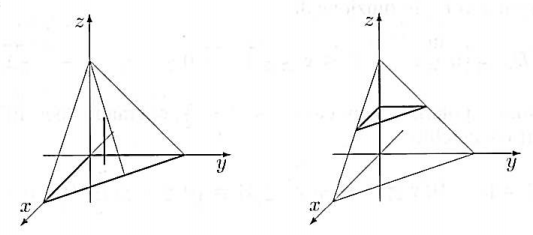
\includegraphics[height=5cm]{../6-integrali doppi e tripli (analisi II)/img2.PNG}
\end{center}
\subsubsection{Equazione di un piano passante per tre punti}
L'equazione caratteristica di un piano è $ax + bx + cz = d$, dati i tre punti $(x_1,y_1,z_1), (x_2,y_2,z_2), (x_3,y_3,z_3)$ scriviamo il sistema:
\[
    \begin{cases}
        a x_1 + by_1 + c z_1 = d\\
        a x_2 + by_2 + c z_2 = d\\
        a x_3 + by_3 + c z_3 = d
    \end{cases}
\]
da cui ricaviamo i valori di $a,b,c$ e $d$ da sostituire.\newline
\newline
C'è anche quest'altro metodo ma non ne sono sicurissimo:\newline
Piano per tre punti $(x_a, y_a, z_a)$ $(x_b, y_b, z_b)$ e $(x_c, y_c, z_c)$ è il determinante della matrice 
\[
    det\left(\begin{matrix}
        x-x_a & y-y_a & z-z_a\\
        x_b-x_a & y_b-y_a & z_b-z_a\\
        x_c-x_a & y_c - y_a & z_c -z_a 
    \end{matrix}\right) = 0
\]
\subsubsection{Equazioni di circonferenze non centrate nell'origine}
La generica equazione della circonferenza è
\[
    (x-x_c)^2 + (y-y_c)^2 = r
\]
in cui $(x_c, y_c)$ sono le coordinate della circonferenza e $r$ è il raggio.\newline
\newline
Spesso negli esercizi si trovano equazioni come per esempio $x^2 + y^2 -2y = 0$, per capire come è fatta è sufficiente sviluppare l'equazione generica della ciroconferenza e eguagliare i termini per capire il centro e il raggio:
\[
    x^2 + x_c^2 -2x_cx + y^2 + y_c^2 - 2y_cy - r = 0
\]
da cui concludiamo che $y_c = 1$ e $x_c = 0$ e $r=1$.